% !TEX root = ../thesis.tex

In this final set of simulations, we will have a look on behavior at higher Reynolds numbers.

But first of all, we need to introduce a model concept for 2D vortices.

\subsubsection{The Rankine vortex}
\label{subs:The Rankine vortex}

For the final set of simulations, we introduce the Rankine-vortex.
It is an idealized model of a vortex, satisfying the Navier-Stokes equations, c.f.~\cite{tryggeson2007analytical} and mixing the definitions of a rigid body vortex\footnote{A rigid body vortex has constant vorticity and radially increasing velocities, like the eponymic spinning rigid body.}
in the inner region and a potential vortex\footnote{The vorticity of a potential vortex is equal to the delta distribution $\delta$, c.f.~\eqref{eq: diraque feature}, the graph of the velocity is hyperbolic.} in the outer region.


\begin{figure}[h!]
\centering
\begin{subfigure}[b]{.5\textwidth}
  \centering
  % !TEX root = ../../thesis.tex

\begin{tikzpicture}
  \begin{axis}[
  axis x line=center,
  axis y line=center,
  xtick={-5,-4,...,5},
  ytick={-1,-0.5,...,1},
  xmin=-5.5,
  xmax=6.5,
  ymin=-1.2,
  ymax=1.5,
  x post scale=1.6,
  y post scale=0.7,
  xlabel=$x$,
  ylabel=$u_y$,
  samples=200]
  \addplot[blue,domain=1:5] {1/x};
  \addplot[blue,domain=-5:-1] {1/x};
  \addplot[blue,domain=-1:1] {x};
  \end{axis}
\end{tikzpicture}

  \caption{$y$-velocity}
\label{fig: rankine velocity}
\end{subfigure}%
\begin{subfigure}[b]{.5\textwidth}
  \centering
  % !TEX root = ../../thesis.tex

\begin{tikzpicture}
  \begin{axis}[
  axis x line=center,
  axis y line=center,
  xtick={-1,...,1},
  ytick={0,1},
  xmin=-5.5,
  xmax=6.5,
  ymin=-1.2,
  ymax=1.5,
  x post scale=1,
  y post scale=0.7,
  xlabel=$x$,
  ylabel=$vorticity$,
  samples=200]

  \addplot[blue,thick,domain=1:5] {0};
  \addplot[blue,thick,domain=-5:-1] {0};
  \addplot[blue,thick,domain=-1:1] {1};
  \addplot[color=blue, thick,dashed] coordinates {
                    (1, 0)
                    (1,1)
                };
  \addplot[color=blue, thick,dashed] coordinates {
                    (-1, 0)
                    (-1,1)
                };
  \fill [fill=white] (axis cs:-0.2,-2.2) rectangle (axis cs:0.2,-0.05);
  \node at (axis cs:0.01,-0.23) {$0$};
  \end{axis}
\end{tikzpicture}

  \caption{vorticity}
\label{fig: rankine vorticity}
\end{subfigure}
\caption{Cut through the middle of a Rankine vortex.
The inner part is a rigid body vortex with constant vorticity, whereas the outer part is a potential vortex which is vorticity free in this area.}
\label{fig: rankine}
\end{figure}

Figure~\ref{fig: rankine} shows the $y$ component of the velocity and the vorticity when cutting through a Rankine vortex at $y=0$, the $x$ component is zero.
A more thorough treatment can be found in~\cite{giaiotti2006rankine} amongst others.

\begin{figure}
  \centering
  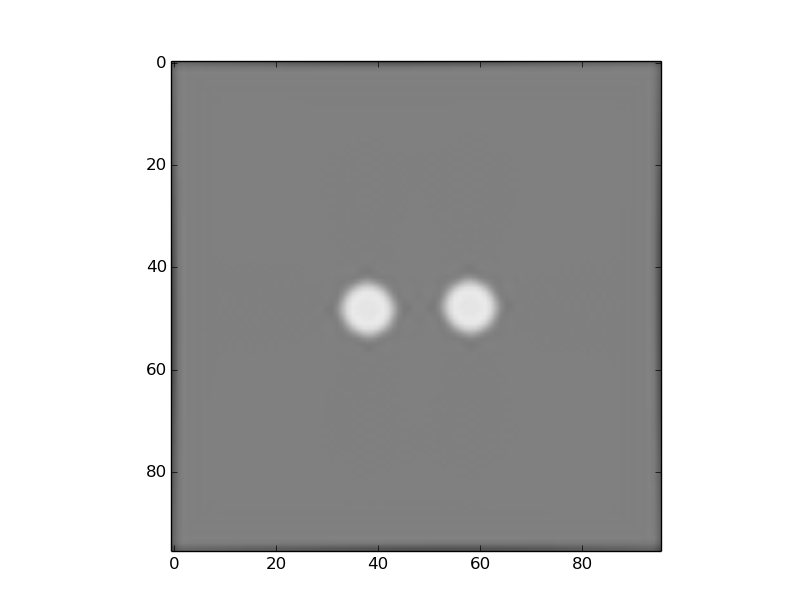
\includegraphics[width=0.6\textwidth]{../figures/rankine_vortex.png}  % chktex 11
  \caption{Setup for the vortex merge simulation on a $96^2$ grid. White is positive and black negative vorticity.}
\label{fig: vortex merge setup}
\end{figure}

\subsubsection{Simulation setup and goals}
\label{subs:Simulation setup and goals}

Figure~\ref{fig: vortex merge setup} depicts the simplest nontrivial setting consisting of two vortices next to each other with the same direction of rotation, in our case counterclockwise, i.e.\ with positive vorticity.
Additionally, we have a periodic domain, hence need not to deal with any sorts of boundaries and no force terms.

Two things are expected to happen.
Despite the Rankine vortex satisfying Navier-Stokes, there is a kink in the velocity distribution and a jump in vorticity, which will be smoothed out according to the value of the viscosity and hence Reynolds number.
This is described with the Lamb-Oseen vortex\footnote{Also called Hamel-Oseen vortex. Just Orseen vortex for short.} model, c.f.~\cite{tryggeson2007analytical}.

Secondly, the vortices will orbit each other and eventually merge, resulting in one vortex with the same orientation of rotation.

Our goal is now to track the evolution of the vortices and measure when they merge.
To achieve this, we will track the evolution of the enstrophy $\mathcal{E}$, defined as the mean square vorticity
\begin{equation*}
  \label{eq: enstrophy}
  \mathcal{E} \defined \frac{1}{2}\int_{\Omega} \omega^2 \text{dx}
\end{equation*}
where $\Omega$ is the computational domain and $\omega$ is the vorticity\footnote{Unfortunately, $\omega$ is the common notation for vorticity. Not to be confused with the relaxation parameters from the previous sections.}, computed as
\begin{equation*}
  \label{eq: vorticity}
  \omega \defined \partial_x u_y - \partial_y u_x
\end{equation*}
in the two-dimensional setting.

\subsubsection{Results}
\label{subs:Results}

\begin{figure}
  \centering
  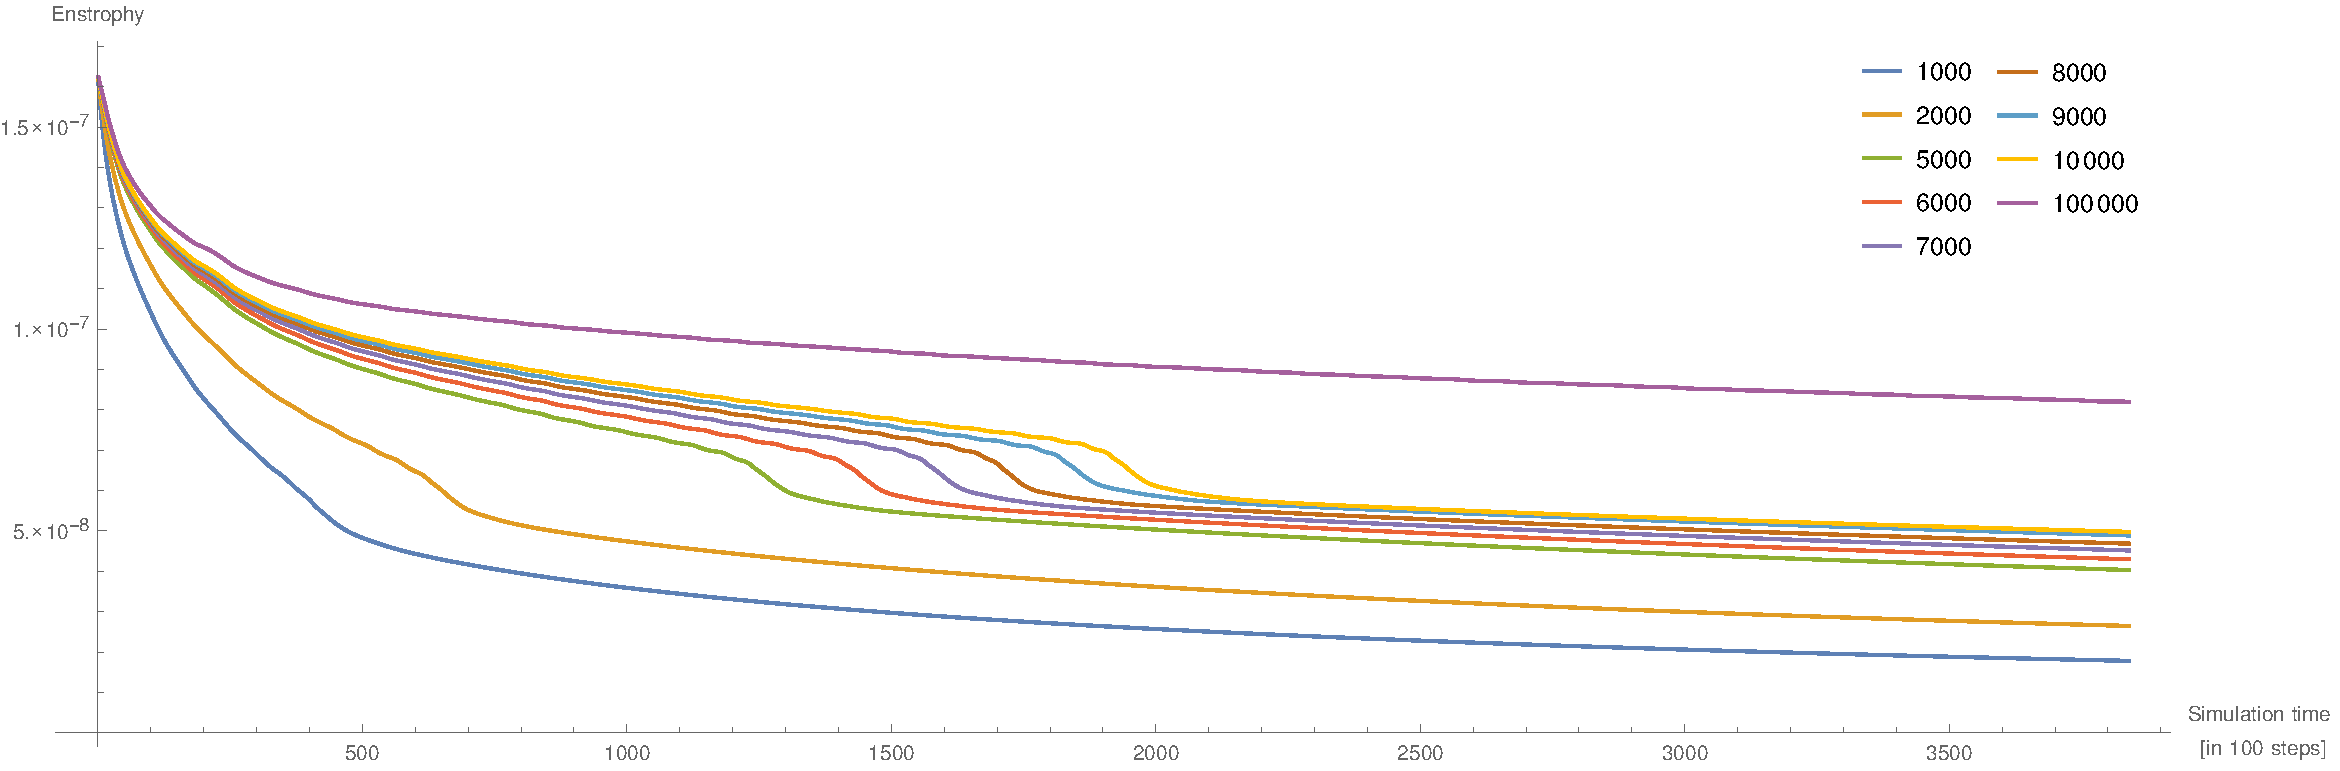
\includegraphics[width=\textwidth]{../figures/vortexMerge_enstrophy_cumulants.pdf}  % chktex 11
  \caption{Evolution of the enstrophy at increasing Reynolds numbers with Cumulant}
\label{fig: rankine cumulant all}
\end{figure}

Figure~\ref{fig: rankine cumulant all} shows the evolution of the enstrophy for different Reynolds numbers.
Its behavior mimics exactly, what we predicted with the thoughts of last section.
First of all we have a steep drop flattening out over time.
This is the behavior expected from the Rankine vortex getting smoothed out to an Orseen vortex which slowly gets bigger and diffuses.
Of course this effect is dragged out, the bigger the Reynolds number is.

After some time however, there is again a steeper passage.
We could suspect this being the time of the merge.

\begin{figure}
  \centering
  \begin{subfigure}[b]{\textwidth}
    \centering
    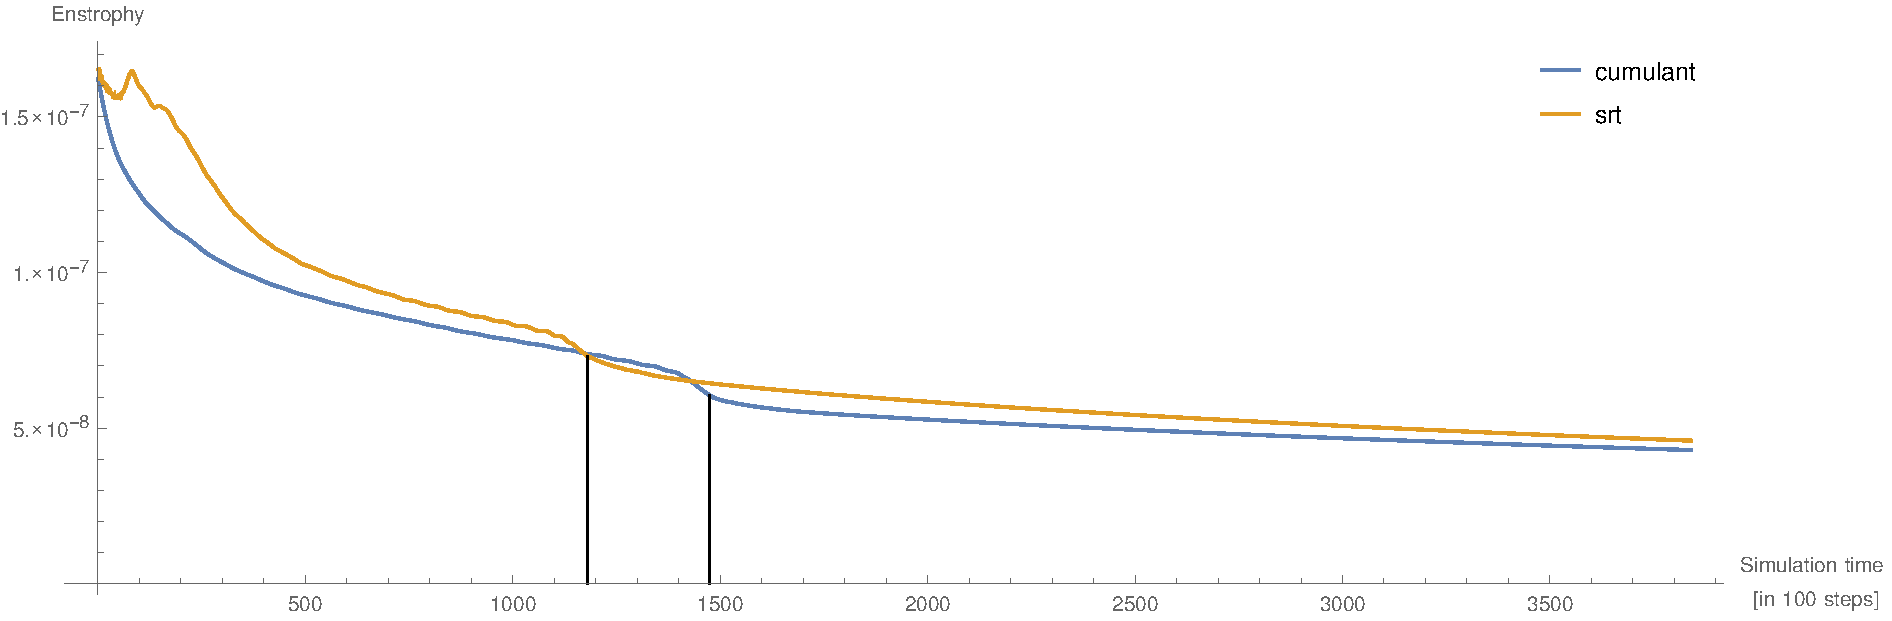
\includegraphics[width=\textwidth]{../figures/vortexMerge_enstrophy.pdf}  % chktex 11
    \caption{Evolution of the enstrophy}
\label{fig: rankine result}
  \end{subfigure}%

  \medskip
  \begin{subfigure}[b]{.5\textwidth}
    \centering
    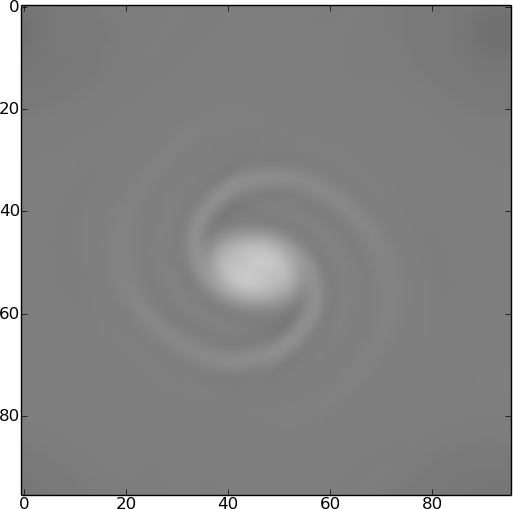
\includegraphics[width=0.6\textwidth]{../figures/cumulant_Re6000_size96_1475.png}  % chktex 11
    \caption{\raggedright{}	Vorticity with Cumulants at timestep $147500$}
\label{fig: rankine cumulant}
  \end{subfigure}\begin{subfigure}[b]{.5\textwidth}
    \centering
    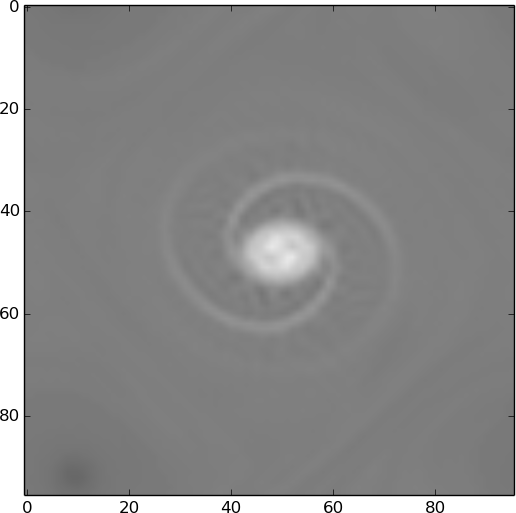
\includegraphics[width=0.6\textwidth]{../figures/srt_Re6000_size96_1181.png}  % chktex 11
    \caption{Vorticity with \gls{srt} at timestep $118100$\newline}
\label{fig: rankine srt}
  \end{subfigure}
  \caption{Simulation of the vortex merging at Reynolds number $6000$}
\label{fig: rankine 6000}
\end{figure}
And indeed, when picking out the simulations for the cumulants ans \gls{srt} at Reynolds number $6000$, illustrated in Figure~\ref{fig: rankine 6000}, we see that this is exactly the moment the two vortices merge.
Also the observed shapes match experimental results, e.g.\ from~\cite{tabeling2002two}, where they gathered many results from 2D turbulence experiments.
On a quick slide in, one should mention, that against common believe, there is such a thing as two-dimensional turbulence\footnote{Which behaves fundamentally different than the three-dimensional counterpart. In 2D, the common pattern are small vortices which merge to large structures where they finally dissipate, in 3D initially large vortices break up until they dissipate at the small scales.}.
It is true, that most initially two-dimensional structures in three-dimensional flows evolve to three-dimensional patterns\footnote{For
example the transition from two-dimensional Tollmien-Schlichting waves to  three-dimensional lambda vortices in the transition of a laminar to a turbulent boundary, c.f.~\cite{knörnschild2001untersuchungen}.},
limiting those studies to real two-dimensional flows.

On comparing the result for Cumulants, Figure~\ref{fig: rankine cumulant} and \gls{srt}, Figure~\ref{fig: rankine srt}, we find more differences.
The \gls{srt} has an unsteady part at the beginning, and also merges way earlier.
Upon looking at the vorticity plot, there are noticeable artifacts around the vortex.

\begin{figure}
  \centering
  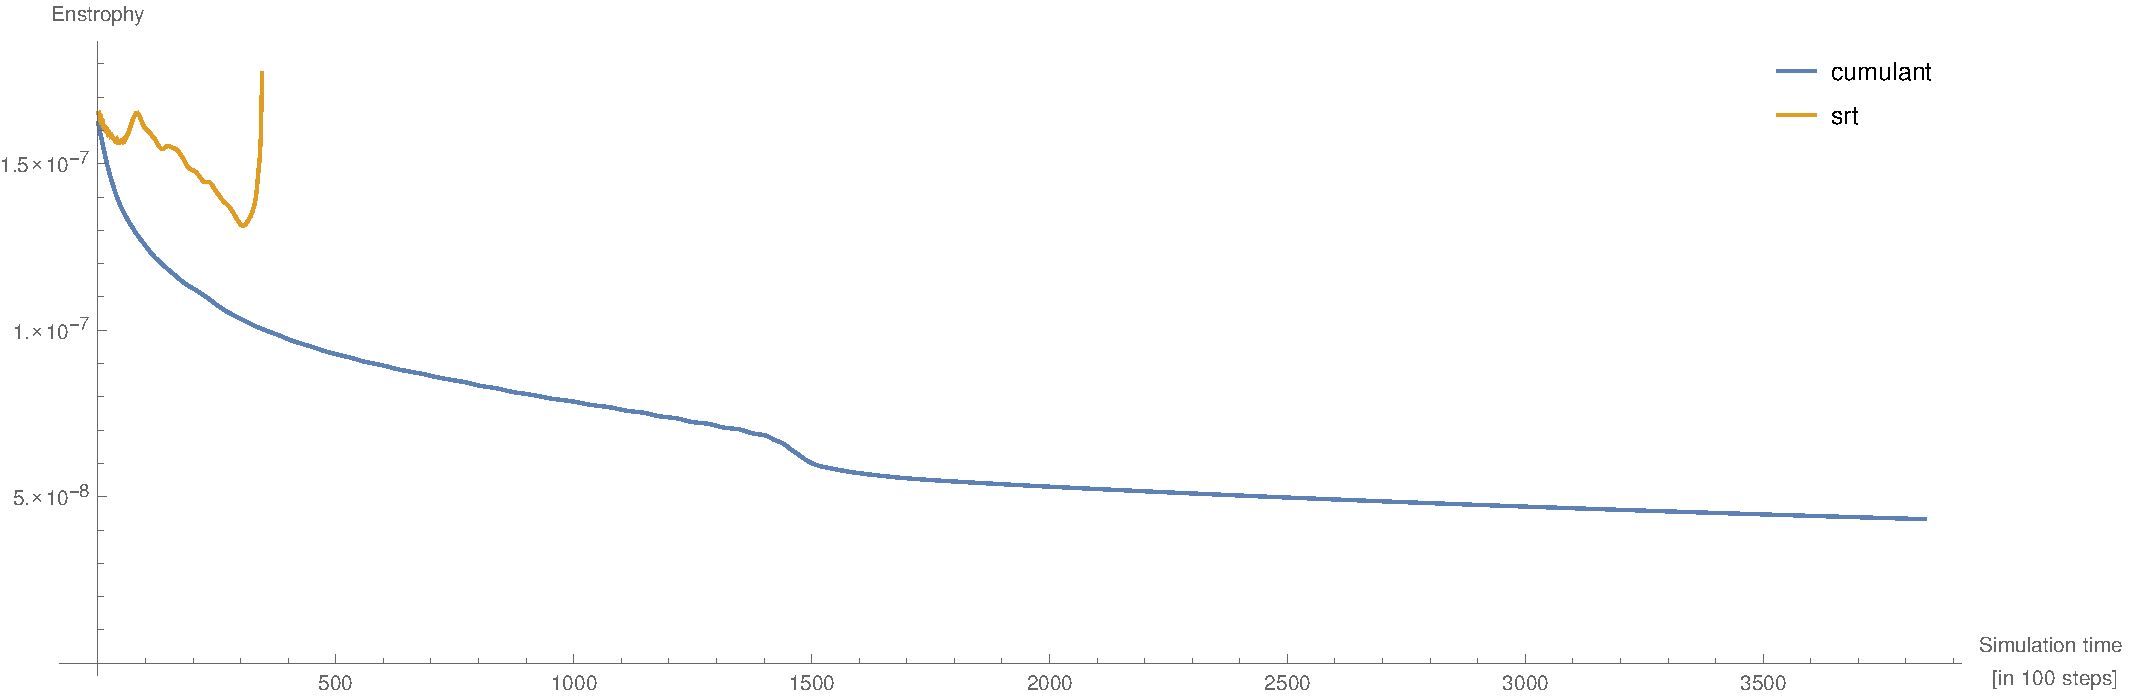
\includegraphics[width=\textwidth]{../figures/vortexMerge_enstrophy6100.pdf}  % chktex 11
  \caption{Evolution of the enstrophy at Reynolds number $6100$}
\label{fig: rankine 6100}
\end{figure}
When amping up the Reynolds number to $6100$, the simulation with \gls{srt} blows up right at the beginning, as shown in Figure~\ref{fig: rankine 6100}.

With this in mind, the results from Figure~\ref{fig: rankine cumulant all} look that much more impressive than they did at the beginning.
